\vzmstitle{ИНТЕГРИРУЕМЫЕ МАТЕМАТИЧЕСКИЕ БИЛЛИАРДЫ В МАГНИТНОМ ПОЛЕ. ТОПОЛОГИЧЕСКИЙ АНАЛИЗ}
\vzmsauthor{Пустовойтов}{С.\,Е.}
\vzmsinfo{Москва; {\it pustovoitovse1@mail.ru}}
\vzmscaption

	Математическим биллиардом называется динамическая система, описывающая движение материальной точки внутри связной, компактной, замкнутой области с кусочно"=гладкой границей. При попадании точки на границу её вектор скорости меняется согласно естественному закону отражения. Далее будем рассматривать плоский биллиард. Для описанной таким образом системы будет иметь место первый интеграл -- полная энергия $H$. Если же у системы будет ещё один первый интеграл $F$, то можно рассмотреть слоение изоэнергетического многообразия $Q^3=\{(x,y,\dot{x}, \dot{y}): H(x,y,\dot{x}, \dot{y})=h\}$ поверхностями уровней интегралов $T^2_{h,f}=\{(x,y,\dot{x}, \dot{y}): H(x,y,\dot{x}, \dot{y})=h, F(x,y,\dot{x}, \dot{y})=f\}$. Для гладких интегрируемых гамильтоновых систем известно, что регулярными слоями $T^2_{h,f}$ являются торы (Теорема Лиувилля). Особыми слоями являются двумерные комплексы -- атомы, описанные и классифицированные А.Т.Фоменко в [1]. Строго говоря, математический биллиард не является гладкой системой. Однако во многих случаях можно показать, что приведённые теоремы и для подобных систем имеют место.

	Рассмотрим плоский биллиард, помещённый в однородное магнитное поле с напряжённостью $B$, линии которого направленны перпендикулярно поверхности стола. Уравнения, описывающие движение единичного заряда, имеют вид
	$$
	\ddot{x} =B\dot{y}
	$$
	$$
	\ddot{y} =-B\dot{x}
	$$
	Отметим, что эти уравнения задают движение по окружности произвольного радиуса с произвольным центром.

	А.Е.Мироновым и М.Бялым в [2] было доказано, что в случае выпуклого односвязного биллиарда интегрируемость имеет место только в случае биллиарда в круге. В таком случае первые интегралы имеют вид

	$$
	H=\dot{x}^2+\dot{y}^2=(BA)^2
	$$
	$$
	F=\frac{\dot{x}^2+\dot{y}^2}{2}+\frac{k}{2}(x^2+y^2)+k(x\dot{y}-y\dot{x})=(BR)^2
	$$
	где $A$--радиус дуги траектории между ударами о стенку, $R$--радиус окружности, точки которой являются центрами дуг траекторий. Пример движения приведён на рисунке ниже.

	\begin{figure}[h!]
		\center{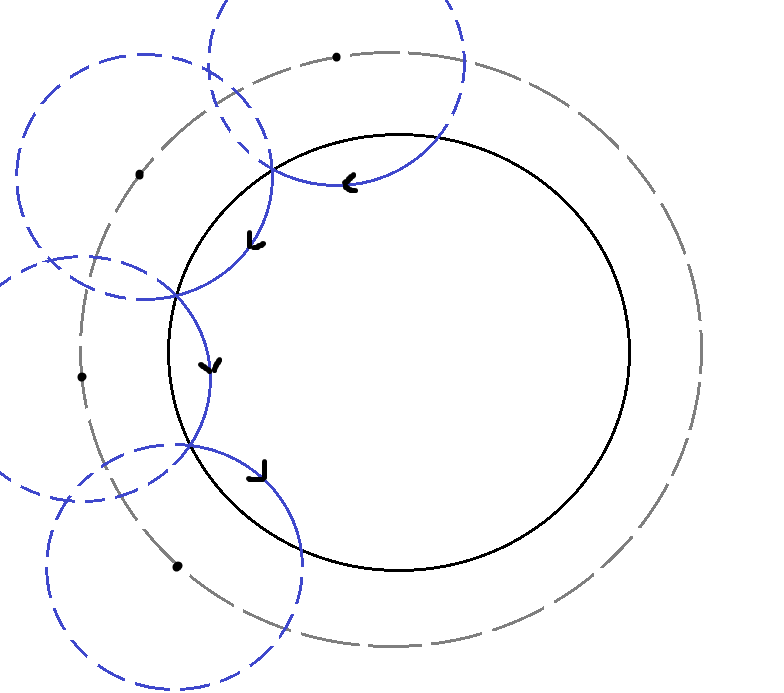
\includegraphics[width=60mm]{ex2}}
		\caption{Пример траектории}
	\end{figure}
	Стоит отметить, что магнитный биллиард в кольце концентрических окружностей также будет интегрируем. Интегралы останутся теми же.

	\textbf{Теорема~1.} {\it В случаях магнитного биллиарда в круге или кольце будет сохраняться теорема Лиувилля, а слоения изоэнергетических многообразий $Q^3$ могут быть описаны полными инвариантами Фоменко-Цишанга.}

	В частности, был получен инвариант, который ранее не встречался для биллиардных систем, но имел место в динамике твёрдого тела.

	В докладе будут приведены бифуркационные диаграммы данных биллиардных систем, представлены все полные инварианты Фоменко-Цишанга, а также приведены динамические системы, Лиувиллево эквивалентные данным.

	Исследование выполнено в рамках Программы Президента Российской Федерации для государственной поддержки ведущих научных школ РФ (грант НШ-2554.2020.1)

	\smallskip \centerline {\bf Литература} \nopagebreak

	1. {\it Болсинов А.В., Фоменко А.Т.} Интегрируемые гамильтоновы системы. Геометрия, топология, классификация. Том I.
	--- Ижевск: РХД, 1999.

	2. {\it M. Bialy, A. E. Mironov} “Algebraic non-integrability of magnetic billiards”,
	J. Phys. A, 49:45 (2016), 455101, 18 pp.

	3. {\it Фокичева В.В.} Топологическая классификация биллиардов в локально плоских областях, ограниченных дугами софокусных квадрик, Матем. сб., 206:10 (2015), 127-176.

	4. {\it М. Бялый, А. Е. Миронов} Полиномиальная неинтегри-
	руемость магнитных бильярдов на сфере и гиперболиче-
	ской плоскости, УМН, 2019, том 74, выпуск 2(446), 3–26
